
\begin{abox}
	Practice set 1
\end{abox}
\begin{enumerate}
	\begin{minipage}{\textwidth}
		\item A plane electromagnetic wave is propagating in a lossless dielectric. The electric field is given by
		$$
		\vec{E}(x, y, z, t)=E_{0}(\hat{x}+A \hat{z}) \exp \left[i k_{0}\{-c t+(x+\sqrt{3} z)\}\right]
		$$
		where $c$ is the speed of light in vacuum, $E_{0}, A$ and $k_{0}$ are constant and $\hat{x}$ and $\hat{z}$ are unit vectors along the $x$-and $z$-axes. The relative dielectric constant of the medium $\varepsilon_{r}$ and the constant $A$ are
		\exyear{NET JUNE 2011}
	\end{minipage}
	\begin{tasks}(2)
		\task[\textbf{a.}]$\varepsilon_{r}=4$ and $A=-\frac{1}{\sqrt{3}}$
		\task[\textbf{b.}]$\varepsilon_{r}=4$ and $A=+\frac{1}{\sqrt{3}}$
		\task[\textbf{c.}]$\varepsilon_{r}=4$ and $A=\sqrt{3}$
		\task[\textbf{d.}]$\varepsilon_{r}=4$ and $A=-\sqrt{3}$
	\end{tasks}
\begin{answer}
	\begin{align*}
	\vec{E}(x, y, z, t)&=E_{0}(\hat{x}+A \hat{z}) \exp \left[i k_{0}\{-c t+(x+\sqrt{3} z)\}\right]\\
	\text{Comparing with term }e^{i(\vec{k}, \vec{r}-\alpha x)} \Rightarrow \vec{k}&=k_{0}(\hat{x}+\sqrt{3} \hat{z})\text{ and }\omega=k_{0} c.\\
	\text{Since }v&=\frac{\omega}{k}=\frac{k_{0} c}{\sqrt{k_{0}^{2}+3 k_{0}^{2}}}=\frac{c}{2} \Rightarrow\text{ Refractive index }n\\&=\sqrt{\varepsilon_{r}}=2 \Rightarrow \varepsilon_{r}=4.\\
	\text{Since }\vec{k} \cdot \hat{n}&=0 \Rightarrow k_{0}(\hat{x}+\sqrt{3} \hat{z}) \cdot(\hat{x}+A \hat{z})\\&=0 \Rightarrow k_{0}(1+A \sqrt{3})=0 \Rightarrow A=-\frac{1}{\sqrt{3}}
	\end{align*}
	So the correct answer is \textbf{Option (c)}
\end{answer}
	\begin{minipage}{\textwidth}
		\item The magnetic field of the $T E_{11}$ mode of a rectangular waveguide of dimensions $a \times b$ as shown in the figure is given by $H_{z}=H_{0} \cos (0.3 \pi x) \cos (0.4 \pi y)$, where $x$ and $y$ are in cm
		\exyear{NET JUNE 2011}
		\begin{figure}[H]
			\centering
			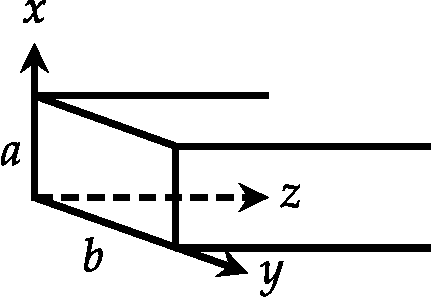
\includegraphics[height=3cm,width=5cm]{diagram-20211011(7)-crop}
		\end{figure}
	\end{minipage}
	$\text { A. The dimensions of the waveguide are }$
	\begin{tasks}(2)
		\task[\textbf{a.}] $a=3.33 \mathrm{~cm}, b=2.50 \mathrm{~cm}$
		\task[\textbf{b.}]$a=0.40 \mathrm{~cm}, b=0.30 \mathrm{~cm}$
		\task[\textbf{c.}]$a=0.80 \mathrm{~cm}, b=0.60 \mathrm{~cm}$
		\task[\textbf{d.}] $a=1.66 \mathrm{~cm}, b=1.25 \mathrm{~cm}$
	\end{tasks}
	\begin{answer}
		\begin{align*}
		\text{Since }H_{z}&=H_{0} \cos (0.3 \pi x) \cos (0.4 \pi y)\\
		\Rightarrow \frac{m \pi}{a}&=0.3 \pi\text{ where }\mathrm{m}=1\text{ and }\frac{\mathrm{n} \pi}{\mathrm{b}}=0.4 \pi\text{ where }\mathrm{n}=1\\
		\Rightarrow a&=3.33 \mathrm{~cm}, b=2.50 \mathrm{~cm}
		\end{align*}
		So the correct answer is \textbf{Option (a)}
	\end{answer}
	\begin{minipage}{\textwidth}
		\item An electromagnetic wave is incident on a water-air interface. The phase of the perpendicular component of the electric field, $E_{\perp}$, of the reflected wave into the water is found to remain the same for all angles of incidence. The phase of the magnetic field $H$
		\exyear{NET JUNE 2012}
	\end{minipage}
	\begin{tasks}(2)
		\task[\textbf{a.}]does not change
		\task[\textbf{b.}]changes by $3 \pi / 2$
		\task[\textbf{c.}]changes by $\pi / 2$
		\task[\textbf{d.}]changes by $\pi$
	\end{tasks}
	\begin{answer}
		So the correct answer is \textbf{Option (d)}
	\end{answer}
	\begin{minipage}{\textwidth}
		\item A current $I$ is created by a narrow beam of protons moving in vacuum with constant velocity $\vec{u}$. The direction and magnitude, respectively of the Poynting vector $\vec{S}$ outside the beam at a radial distance $r$ (much larger than the width of the beam) from the axis, are
		\exyear{NET JUNE 2013}
	\end{minipage}
	\begin{tasks}(2)
		\task[\textbf{a.}] $\vec{S} \perp \vec{u}$ and $|\vec{S}|=\frac{I^{2}}{4 \pi^{2} \varepsilon_{0}|\vec{u}| r^{2}}$
		\task[\textbf{b.}]$\vec{S} \|(-\vec{u})$ and $|\vec{S}|=\frac{I^{2}}{4 \pi^{2} \varepsilon_{0}|\vec{u}| r^{4}}$
		\task[\textbf{c.}]$\vec{S} \| \vec{u}$ and $|\vec{S}|=\frac{I^{2}}{4 \pi^{2} \varepsilon_{0}|\vec{u}| r^{2}}$
		\task[\textbf{d.}]$\vec{S} \| \vec{u}$ and $|\vec{S}|=\frac{I^{2}}{4 \pi^{2} \varepsilon_{0}|\vec{u}| r^{4}}$
	\end{tasks}
\begin{answer}
	\begin{align*}
	\intertext{Let charge per unit length be $\lambda$, hence $I=\lambda u$ in $z$-direction.}
	\text{The magnetic field at a distance $r$ is }\vec{B}&=\frac{\mu_{0} I}{2 \pi r} \hat{\phi}.\\
	\text{The electric field at a distance $r$ is }\vec{E}&=\frac{\lambda}{2 \pi \varepsilon_{0} r} \hat{r}=\frac{I}{2 \pi \varepsilon_{0} u r} \hat{r}.\\
	\text{Hence Poynting vector }\vec{S}&=\frac{\vec{E} \times \vec{B}}{\mu_{0}}=\frac{I^{2}}{4 \pi^{2} \varepsilon_{0} u r^{2}} \hat{z}
	\end{align*}
	So the correct answer is \textbf{Option (c)}
\end{answer}
	\begin{minipage}{\textwidth}
		\item The electric field of an electromagnetic wave is given by
		$$
		\vec{E}=E_{0} \cos [\pi(0.3 x+0.4 y-1000 t)] \hat{k} .
		$$
		The associated magnetic field $\vec{B}$ is
		\exyear{NET DEC 2013}
	\end{minipage}
	\begin{tasks}(1)
		\task[\textbf{a.}] $10^{-3} E_{0} \cos [\pi(0.3 x+0.4 y-1000 t)] \hat{k}$
		\task[\textbf{b.}]$10^{-4} E_{0} \cos [\pi(0.3 x+0.4 y-1000 t)](4 \hat{i}-3 \hat{j})$
		\task[\textbf{c.}]$E_{0} \cos [\pi(0.3 x+0.4 y-1000 t)](0.3 \hat{i}+0.4 \hat{j})$
		\task[\textbf{d.}]$10^{2} E_{0} \cos [\pi(0.3 x+0.4 y-1000 t)](3 \hat{i}+4 \hat{j})$
	\end{tasks}
\begin{answer}
	\begin{align*}
	\vec{k}&=\pi(0.3 \hat{x}+0.4 \hat{y}), \omega=1000 \pi\\
	\vec{B}&=\frac{\vec{k} \times \vec{E}}{\omega}=\frac{1}{\omega} \pi(0.3 \hat{x}+0.4 \hat{y}) \times E_{0} \cos [\pi(0.3 x+0.4 y-1000 t)] \hat{k}\\
	\Rightarrow \vec{B}&=10^{-4} E_{0} \cos [\pi(0.3 x+0.4 y-1000 t)](4 \hat{i}-3 \hat{j})
	\end{align*}
	So the correct answer is \textbf{Option (b)}
\end{answer}
	\begin{minipage}{\textwidth}
		\item A beam of light of frequency $\omega$ is reflected from a dielectric-metal interface at normal incidence. The refractive index of the dielectric medium is $n$ and that of the metal is $n_{2}=n(1+i \rho)$. If the beam is polarised parallel to the interface, then the phase change experienced by the light upon reflection is
		\exyear{NET JUNE 2014}
	\end{minipage}
	\begin{tasks}(2)
		\task[\textbf{a.}] $\tan (2 / \rho)$ 
		\task[\textbf{b.}]$\tan ^{-1}(1 / \rho)$
		\task[\textbf{c.}]$\tan ^{-1}(2 / \rho)$
		\task[\textbf{d.}]$\tan ^{-1}(2 \rho)$
	\end{tasks}
\begin{answer}
	\begin{align*}
	\text{Since }\tilde{E}_{0 R}&=\left(\frac{1-\tilde{\beta}}{1+\tilde{\beta}}\right) \tilde{E}_{0 I} \\\text{ where }\tilde{\beta}&=\frac{v_{1}}{v_{2}}=\frac{c / n}{c / n(1+i \rho)}=1+i \rho\\
	\Rightarrow \tilde{E}_{0 R}&=\left(\frac{-i \rho}{2+i \rho}\right) \tilde{E}_{0 I}=\left(\frac{\rho e^{-i \pi / 2}}{\sqrt{4+\rho^{2}} e^{i \theta}}\right) \tilde{E}_{0 I}\\&=\left(\frac{\rho}{\sqrt{4+\rho^{2}}}\right) e^{-i(\pi / 2+\theta)} \tilde{E}_{0 I}\text{ where }\tan \theta=\frac{\rho}{2}\\
	\text{Thus phase change }\phi&=-(\pi / 2+\theta) \Rightarrow \tan \phi=\cot \theta\\&=\frac{2}{\rho} \Rightarrow \phi=\tan ^{-1}\left(\frac{2}{\rho}\right)
	\end{align*}
	So the correct answer is \textbf{Option (c)}
\end{answer}
	\begin{minipage}{\textwidth}
		\item An electromagnetically-shielded room is designed so that at a frequency $\omega=10^{7} \mathrm{rad} / \mathrm{s}$ the intensity of the external radiation that penetrates the room is $1 \%$ of the incident radiation. If $\sigma=\frac{1}{2 \pi} \times 10^{6}(\Omega m)^{-1}$ is the conductivity of the shielding material, its minimum thickness should be (given that $\ln 10=2.3$ )
		\exyear{NET JUNE 2014}
	\end{minipage}
	\begin{tasks}(2)
		\task[\textbf{a.}] $4.60 \mathrm{~mm}$
		\task[\textbf{b.}]$2.30 \mathrm{~mm}$
		\task[\textbf{c.}] $0.23 \mathrm{~mm}$
		\task[\textbf{d.}]$0.46 \mathrm{~mm}$
	\end{tasks}
\begin{answer}
	\begin{align*}
	I&=I_{0} e^{-2 \kappa z} \Rightarrow z=\frac{1}{2 \kappa} \ln \left(\frac{I_{0}}{I}\right)\\
	\text{where }\frac{I_{0}}{I}&=100, \kappa=\sqrt{\frac{\sigma \mu \omega}{2}}=\sqrt{\frac{1}{2} \times \frac{1}{2 \pi} \times 10^{6} \times 4 \pi \times 10^{-7} \times 10^{7}}=10^{3}\\
	\Rightarrow z&=\frac{1}{2 \times 10^{3}} \ln (100)=2.30 \mathrm{~mm}
	\end{align*}
	So the correct answer is \textbf{Option (b)}
\end{answer}
	\begin{minipage}{\textwidth}
		\item A plane electromagnetic wave incident normally on the surface of a material is partially reflected. Measurements on the standing wave in the region in front of the interface such that the ratio of the electric field amplitude at the maxima and the minima is 5 . The ratio of the reflected intensity to the incident intensity is
		\exyear{NET JUNE 2014}
	\end{minipage}
	\begin{tasks}(4)
		\task[\textbf{a.}] $4 / 9$
		\task[\textbf{b.}] $2 / 3$
		\task[\textbf{c.}]$2 / 5$
		\task[\textbf{d.}]$1 / 5$
	\end{tasks}
\begin{answer}
	\begin{align*}
	\frac{E_{0 I}+E_{0 R}}{E_{0 I}-E_{0 R}}&=5 \Rightarrow E_{0 I}+E_{0 R}=5\left(E_{0 I}-E_{0 R}\right) \\&\Rightarrow 6 E_{0 R}=4 E_{0 I} \Rightarrow \frac{E_{0 R}}{E_{0 I}}=\frac{2}{3}\\
	&\Rightarrow \frac{I_{R}}{I_{I}}=\left(\frac{E_{0 R}}{E_{0 I}}\right)^{2}=\frac{4}{9}
	\end{align*}
	So the correct answer is \textbf{Option (a)}
\end{answer}
	\begin{minipage}{\textwidth}
		\item A Plane electromagnetic wave is travelling along the positive $z$-direction. The maximum electric field along the $x$ - direction is $10 \mathrm{~V} / \mathrm{m}$. The approximate maximum values of the power per unit area and the magnetic induction $B$, respectively, are
		\exyear{NET JUNE 2015}
	\end{minipage}
	\begin{tasks}(1)
		\task[\textbf{a.}] $3.3 \times 10^{-7}$ watts $/ \mathrm{m}^{2}$ and 10 tesla
		\task[\textbf{b.}]$3.3 \times 10^{-7}$ watts $/ \mathrm{m}^{2}$ and $3.3 \times 10^{-8}$ tesla
		\task[\textbf{c.}]$0.265$ watts / m $^{2}$ and 10 tesla
		\task[\textbf{d.}]$0.265$ watts $/ m^{2}$ and $3.3 \times 10^{-8}$ tesla	
	\end{tasks}
\begin{answer}
	\begin{align*}
	E_{0}&=10 \mathrm{~V} / \mathrm{m}, I=\frac{P}{A}=\frac{1}{2} c \in_{0} E_{0}^{2}\\&=\frac{1}{2} \times 3 \times 10^{8} \times 8.86 \times 10^{-12} \times(10)^{2}=0.132 \mathrm{~W} / \mathrm{m}^{2}\\
	B_{0}&=\frac{E_{0}}{c}=\frac{10}{3 \times 10^{8}}=3.3 \times 10^{-8}\text{ Tesla}
	\end{align*}
	So the correct answer is \textbf{Option (d)}
\end{answer}
	\begin{minipage}{\textwidth}
		\item Consider a rectangular wave guide with transverse dimensions $2 m \times 1 m$ driven with an angular frequency $\omega=10^{9} \mathrm{rad} / \mathrm{s}$. Which transverse electric $(T E)$ modes will propagate in this wave guide?
		\exyear{NET JUNE 2015}
	\end{minipage}
	\begin{tasks}(2)
		\task[\textbf{a.}] $T E_{10}, T E_{01}$ and $T E_{20}$
		\task[\textbf{b.}]$T E_{01}, T E_{11}$ and $T E_{20}$
		\task[\textbf{c.}]$T E_{01}, T E_{10}$ and $T E_{11}$
		\task[\textbf{d.}]$T E_{01}, T E_{10}$ and $T E_{22}$
	\end{tasks}
\begin{answer}
	\begin{align*}
	\omega_{m n}&=C \pi \sqrt{\frac{m^{2}}{a^{2}}+\frac{n^{2}}{b^{2}}}\\
	\omega_{10}&=\frac{c \pi}{a}=\frac{3 \times 10^{8} \times 3.14}{2}=4.71 \times 10^{8} \mathrm{rod} / \mathrm{sec}\\
	\omega_{01}&=\frac{c \pi}{b}=\frac{3 \times 10^{8} \times 3.14}{1}=9.42 \times 10^{8} \mathrm{rod} / \mathrm{sec}\\
	\omega_{11}&=c \pi \sqrt{\frac{1}{a^{2}}+\frac{1}{b^{2}}}=10.53 \times 10^{8} \mathrm{rod} / \mathrm{sec}\\
	\omega_{20}&=\frac{2 c \pi}{a}=9.72 \times 10^{8} \mathrm{rod} / \mathrm{sec}\\
	\omega_{22}&=c \pi \sqrt{\frac{4}{a^{2}}+\frac{4}{b^{2}}}=10.5 \times 10^{8} \mathrm{rod} / \mathrm{sec}\\
	\text{Since }&\omega>\omega_{10}, \omega_{01}, \omega_{20}
	\end{align*}
	So the correct answer is \textbf{Option (a)}
\end{answer}
	\begin{minipage}{\textwidth}
		\item The electric and magnetic fields in the charge free region $z>0$ are given by
		$$
		\begin{aligned}
		&\vec{E}(\vec{r}, t)=E_{0} e^{-k_{1} z} \cos \left(k_{2} x-\omega t\right) \hat{j} \\
		&\vec{B}(\vec{r}, t)=\frac{E_{0}}{\omega} e^{-k_{1} z}\left[k_{1} \sin \left(k_{2} x-\omega t\right) \hat{i}+k_{2} \cos \left(k_{2} x-\omega t\right) \hat{k}\right]
		\end{aligned}
		$$
		where $\omega, k_{1}$ and $k_{2}$ are positive constants. The average energy flow in the $x$-direction is
		\exyear{NET JUNE 2015}
	\end{minipage}
	\begin{tasks}(2)
		\task[\textbf{a.}] $\frac{E_{0}^{2} k_{2}}{2 \mu_{0} \omega} e^{-2 k_{1} z}$
		\task[\textbf{b.}]$\frac{E_{0}^{2} k_{2}}{\mu_{0} \omega} e^{-2 k_{1} z}$
		\task[\textbf{c.}]$\frac{E_{0}^{2} k_{1}}{2 \mu_{0} \omega} e^{-2 k_{1} z}$
		\task[\textbf{d.}]$\frac{1}{2} c \in_{0} E_{0}^{2} e^{-2 k_{1} z}$
	\end{tasks}
	\begin{answer}
		\begin{align*}
		\vec{S}&=\frac{1}{\mu_{0}}(\vec{E} \times \vec{B})=\frac{E_{0}^{2} e^{-2 k_{1} z}}{\mu_{0} \omega}\left[k_{1} \cos \theta \sin \theta(-\hat{k})+k_{2} \cos ^{2} \theta \hat{i}\right]\\\text{, where }\theta&=k_{2} x-\omega t\\
		\Rightarrow \quad\langle\vec{S}\rangle&=\frac{k_{2}}{2} \frac{E_{0}^{2} e^{-2 k_{1} z}}{\mu_{0} \omega}=\frac{E_{0}^{2} k_{2}}{2 \mu_{0} \omega} e^{-2 k_{1} z}
		\end{align*}
		So the correct answer is \textbf{Option (a)}
	\end{answer}
	\begin{minipage}{\textwidth}
		\item A waveguide has a square cross-section of side $2 a$. For the $T M$ modes of wave vector $k$, the transverse electromagnetic modes are obtained in terms of a function $\psi(x, y)$ which obeys the equation
		$$
		\left[\frac{\partial^{2}}{\partial x^{2}}+\frac{\partial^{2}}{\partial y^{2}}+\left(\frac{\omega^{2}}{c^{2}}-k^{2}\right)\right] \psi(x, y)=0
		$$
		with the boundary condition $\psi(\pm a, y)=\psi(x, \pm a)=0$. The frequency $\omega$ of the lowest mode is given by
		\exyear{NET JUNE 2016}
	\end{minipage}
	\begin{tasks}(2)
		\task[\textbf{a.}] $\omega^{2}=c^{2}\left(k^{2}+\frac{4 \pi^{2}}{a^{2}}\right)$
		\task[\textbf{b.}]$\omega^{2}=c^{2}\left(k^{2}+\frac{\pi^{2}}{a^{2}}\right)$
		\task[\textbf{c.}]$\omega^{2}=c^{2}\left(k^{2}+\frac{\pi^{2}}{2 a^{2}}\right)$
		\task[\textbf{d.}]$\omega^{2}=c^{2}\left(k^{2}+\frac{\pi^{2}}{4 a^{2}}\right)$
	\end{tasks}
\begin{answer}
	\begin{align*}
	c^{2} k^{2}&=\omega^{2}-\omega_{m n}^{2} \Rightarrow \omega^{2}=c^{2} k^{2}+\omega_{m n}^{2}\\
	\Rightarrow \omega_{m n}^{2}&=c^{2} \pi^{2}\left(\frac{m^{2}}{a^{2}}+\frac{n^{2}}{b^{2}}\right) \Rightarrow \omega_{11}^{2}=c^{2} \pi^{2}\left[\frac{1}{(2 a)^{2}}+\frac{1}{(2 a)^{2}}\right]\\
	\Rightarrow \omega_{11}^{2}&=c^{2} \pi^{2} \times \frac{1}{2 a^{2}}=\frac{c^{2} \pi^{2}}{2 a^{2}} \Rightarrow \omega^{2}=c^{2}\left(k^{2}+\frac{\pi^{2}}{2 a^{2}}\right)
	\end{align*}
	So the correct answer is \textbf{Option (c)}
\end{answer}
	\begin{minipage}{\textwidth}
		\item An electromagnetic wave (of wavelength $\lambda_{0}$ in free space) travels through an absorbing medium with dielectric permittivity given by $\varepsilon=\varepsilon_{R}+i \varepsilon_{I}$ where $\frac{\varepsilon_{I}}{\varepsilon_{R}}=\sqrt{3}$. If the skin depth is $\frac{\lambda_{0}}{4 \pi}$, the ratio of the amplitude of electric field $E$ to that of the magnetic field $B$, in the medium (in ohms) is
		\exyear{NET JUNE 2017}
	\end{minipage}
	\begin{tasks}(4)
		\task[\textbf{a.}] $120 \pi$
		\task[\textbf{b.}]377
		\task[\textbf{c.}]$30 \sqrt{2} \pi$
		\task[\textbf{d.}] $30 \pi$
	\end{tasks}\begin{answer}
	\begin{align*}
	d&=\frac{1}{\chi}=\frac{\lambda_{0}}{4 \pi}, \frac{\epsilon_{I}}{\epsilon_{R}}=\sqrt{3}=\frac{\sigma}{\omega \in}\\
	\chi&=\omega \sqrt{\frac{\epsilon \mu}{2}}\left[\sqrt{1+\left(\frac{\sigma}{\omega \in}\right)^{2}}-1\right]^{1 / 2} \Rightarrow \chi\\&=\omega \sqrt{\frac{\epsilon \mu}{2}}=\frac{4 \pi}{\lambda_{0}} \Rightarrow \sqrt{\in \mu}=\frac{\sqrt{2}}{\omega} \frac{4 \pi}{\lambda_{0}}\\
	K&=\sqrt{k^{2}+\chi^{2}}=\omega\left[\in \mu \sqrt{1+\left(\frac{\sigma}{\omega \in}\right)^{2}}\right]^{1 / 2}\\
	\frac{E_{0}}{B_{0}}&=\frac{\omega}{K}=\frac{\omega}{\omega\left[\in \mu \sqrt{1+\left(\frac{\sigma}{\omega \in}\right)^{2}}\right]^{1 / 2}}\\&=\frac{1}{\sqrt{2 \in \mu}}=\frac{1}{\sqrt{2} \times \frac{\sqrt{2}}{\omega} \times \frac{4 \pi}{\lambda_{0}}}\\
	&=\frac{\lambda_{0} \omega}{8 \pi}=\frac{\lambda_{0} \times 2 \pi c / \lambda_{0}}{8 \pi}=\frac{c}{4} \Rightarrow \frac{E}{H_{0}}=\frac{c}{4} \mu_{0}\\
	\Rightarrow \frac{E}{H_{0}}&=\frac{4 \pi \times 10^{-7} \times 3 \times 10^{8}}{4}=30 \pi
	\end{align*}
	So the correct answer is \textbf{Option (d)}
\end{answer}
	\begin{minipage}{\textwidth}
		\item An electromagnetic wave is travelling in free space (of permittivity $\varepsilon_{0}$ ) with electric field
		$$
		\vec{E}=\hat{k} E_{0} \cos q(x-c t)
		$$
		The average power (per unit area) crossing planes parallel to $4 x+3 y=0$ will be
		\exyear{NET DEC 2017}
	\end{minipage}
	\begin{tasks}(4)
		\task[\textbf{a.}] $\frac{4}{5} \varepsilon_{0} c E_{0}^{2}$
		\task[\textbf{b.}]$\varepsilon_{0} c E_{0}^{2}$
		\task[\textbf{c.}]$\frac{1}{2} \varepsilon_{0} c E_{0}^{2}$
		\task[\textbf{d.}] $\frac{16}{25} \varepsilon_{0} c E_{0}^{2}$
	\end{tasks}
	\begin{answer}$\left. \right. $
		\begin{figure}[H]
			\centering
			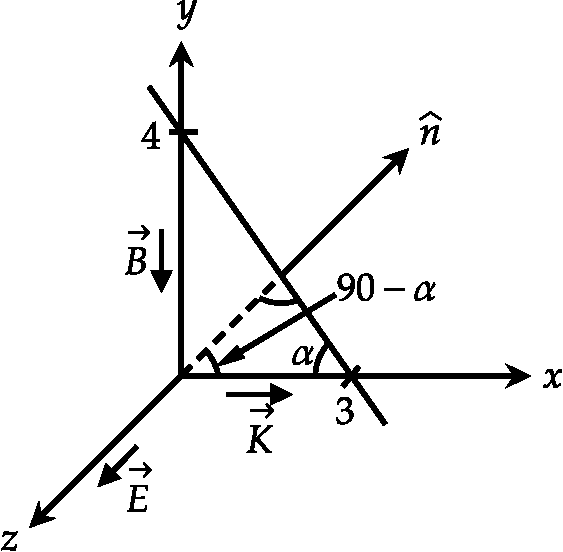
\includegraphics[height=5cm,width=5.5cm]{diagram-20211011(57)-crop}
		\end{figure}
		\begin{align*}
		4 x+3 y&=0 \Rightarrow \frac{x}{3}+\frac{y}{4}=0\\
		\vec{B}&=-\frac{E_{0}}{c} \cos (q x-q c t) \hat{y}\\
		\vec{S}&=\frac{1}{\mu_{0}}(\vec{E} \times \vec{B})=\frac{1}{\mu_{0}}\left(E_{0} \times \frac{E_{0}}{c} \cos ^{2} \theta\right) \hat{x} \Rightarrow\langle\vec{S}\rangle=\frac{E_{0}^{2}}{2 \mu_{0} c} \hat{x}\\
		I&=\langle\vec{S}\rangle \hat{n}=\frac{E_{0}^{2}}{2 \mu_{0} c} \cos (90-\alpha)=\frac{E_{0}^{2}}{2 \mu_{0} c} \sin \alpha=\frac{2}{5} c \varepsilon_{0} E_{0}^{2}\\
		\because \tan \alpha&=\frac{4}{3} \Rightarrow \sin \alpha=\frac{4}{5}\\
		I &\approx 0.4 c \varepsilon_{0} E_{0}^{2} \approx \frac{1}{2} c \varepsilon_{0} E_{0}^{2}
		\end{align*}
		So the correct answer is \textbf{Option (c)}
	\end{answer}
	\begin{minipage}{\textwidth}
		\item A plane electromagnetic wave from within a dielectric medium (with $\varepsilon=4 \varepsilon_{0}$ and $\mu=\mu_{0}$ ) is incident on its boundary with air, at $z=0$. The magnetic field in the medium is $\vec{H}=\hat{j} H_{0} \cos (\omega t-k x-k \sqrt{3} z)$, where $\omega$ and $k$ are positive constants.
		The angles of reflection and refraction are, respectively,
		\exyear{NET DEC 2017}
	\end{minipage}
	\begin{tasks}(4)
		\task[\textbf{a.}] $45^{\circ}$ and $60^{\circ}$
		\task[\textbf{b.}]$30^{\circ}$ and $90^{\circ}$
		\task[\textbf{c.}]$30^{\circ}$ and $60^{\circ}$
		\task[\textbf{d.}]$60^{\circ}$ and $90^{\circ}$
	\end{tasks}
	\begin{answer}$\left. \right. $
		\begin{figure}[H]
			\centering
			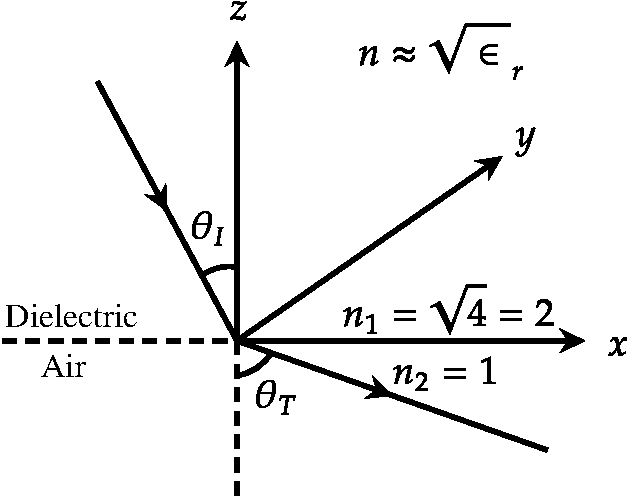
\includegraphics[height=5cm,width=6cm]{diagram-20211011(58)-crop}
		\end{figure}
		\begin{align*}
		n &\approx \sqrt{\epsilon_{r}}\\
		\vec{k}&=k \hat{x}+k \sqrt{3} \hat{z}\\
		\frac{\sin \theta_{I}}{\sin \theta_{T}}&=\frac{n_{2}}{n_{1}}=\frac{1}{2}\\
		\sin \theta_{T}&=2 \sin \theta_{I}\\ \because \tan \theta_{I}&=\frac{k_{x}}{k_{z}}=\frac{1}{\sqrt{3}} \Rightarrow \theta_{1}=30^{\circ}\\
		\Rightarrow \sin \theta_{T}&=2 \times \sin 30^{\circ}=1 \Rightarrow \theta_{T}=90^{\circ}
		\end{align*}
		So the correct answer is \textbf{Option (b)}
	\end{answer}
	\begin{minipage}{\textwidth}
		\item The electric field of a plane wave in a conducting medium is given by
		$$
		\vec{E}(z, t)=\hat{i} E_{0} e^{-z / 3 a} \cos \left(\frac{z}{\sqrt{3} a}-\omega t\right)
		$$
		where $\omega$ is the angular frequency and $a>0$ is a constant. The phase difference between the magnetic field $\vec{B}$ and the electric field $\vec{E}$ is
		\exyear{NET JUNE 2018}
	\end{minipage}
	\begin{tasks}(2)
		\task[\textbf{a.}] $30^{\circ}$ and $\vec{B}$ lags behind $\vec{B}$
		\task[\textbf{b.}]$30^{\circ}$ and $\vec{B}$ lags behind $\vec{E}$
		\task[\textbf{c.}]$60^{\circ}$ and $\vec{E}$ lags behind $\vec{B}$
		\task[\textbf{d.}]$60^{\circ}$ and $\vec{B}$ lags behind $\vec{E}$
	\end{tasks}
\begin{answer}
	\begin{align*}
	\vec{E}(z, t)&=\hat{i} E_{0} e^{-\kappa z} \cos \left(k z-\omega t+\delta_{E}\right) \text{and }\vec{B}(z, t)\\&=\hat{j} B_{0} e^{-\kappa z} \cos \left(k z-\omega t+\delta_{E}+\phi\right)\\
	\text{where }\phi&=\tan ^{-1}\left(\frac{\kappa}{k}\right)\\
	\because \vec{E}(z, t)&=\hat{i} E_{0} e^{-z / 3 a} \cos \left(\frac{z}{\sqrt{3} a}-\omega t\right) \Rightarrow \kappa\\&=\frac{1}{3 a}\text{ and }k=\frac{1}{\sqrt{3} a}\\
	\Rightarrow \phi&=\tan ^{-1}\left(\frac{1}{\sqrt{3}}\right)=30^{\circ}
	\end{align*}
	So the correct answer is \textbf{Option (b)}
\end{answer}
	\begin{minipage}{\textwidth}
		\item A hollow waveguide supports transverse electric $(T E)$ modes with the dispersion relation $k=\frac{1}{c} \sqrt{\omega^{2}-\omega_{m n}^{2}}$, where $\omega_{m n}$ is the mode frequency. The speed of flow of electromagnetic energy at the mode frequency is
		\exyear{NET JUNE 2018}
	\end{minipage}
	\begin{tasks}(4)
		\task[\textbf{a.}] $c$
		\task[\textbf{b.}] $\omega_{m n} / k$
		\task[\textbf{c.}]0
		\task[\textbf{d.}] $\infty$
	\end{tasks}
\begin{answer}
	\begin{align*}
	\intertext{Energy carried by the wave travels at the group velocity}
	v_{g}
	&=\frac{d \omega}{d k}=c \sqrt{1-\left(\frac{\omega_{m n}}{\omega}\right)^{2}} \quad \text{at }omega=\omega_{m n}, v_{g}=0
	\end{align*}
	So the correct answer is \textbf{Option (c)}
\end{answer}
	\begin{minipage}{\textwidth}
		\item In the region far from a source, the time dependent electric field at a point $(r, \theta, \phi)$ is
		$$
		\vec{E}(r, \theta, \phi)=\hat{\phi} E_{0} \omega^{2}\left(\frac{\sin \theta}{r}\right) \cos \left[\omega\left(t-\frac{r}{c}\right)\right]
		$$
		where $\omega$ is angular frequency of the source. The total power radiated (averaged over a cycle) is
		\exyear{NET JUNE 2018}
	\end{minipage}
	\begin{tasks}(4)
		\task[\textbf{a.}] $\frac{2 \pi}{3} \frac{E_{0}^{2} \omega^{4}}{\mu_{0} c}$
		\task[\textbf{b.}]$\frac{4 \pi}{3} \frac{E_{0}^{2} \omega^{4}}{\mu_{0} c}$
		\task[\textbf{c.}]$\frac{4}{3 \pi} \frac{E_{0}^{2} \omega^{4}}{\mu_{0} c}$
		\task[\textbf{d.}]$\frac{2}{3} \frac{E_{0}^{2} \omega^{4}}{\mu_{0} c}$
	\end{tasks}
\begin{answer}
	\begin{align*}
	B&=\frac{E}{c}\\
	|\vec{S}|&=\frac{1}{\mu_{0}} E \cdot B=\frac{E^{2}}{\mu_{0} c}\\&=\frac{E_{0}^{2} \omega^{4}}{\mu_{0} c} \frac{S m_{\theta}^{2}}{r^{2}} \cos ^{2}\left[\omega\left(t-\frac{r}{c}\right)\right]\\
	\langle|\vec{S}|\rangle&=\frac{1}{2} \frac{E_{0}^{2} \omega^{4}}{\mu_{0} c} \frac{\sin ^{2} \theta}{r^{2}}\\
	P&=\oint_{S}\langle|\vec{S}|\rangle \cdot d \vec{a}=\frac{E_{0}^{2} \omega^{4}}{2 \mu_{0} c} \int_{0}^{\pi} \int_{0}^{2 \pi} \frac{\sin ^{2} \theta}{r^{2}} r^{2} \sin \theta d \theta d \phi\\
	P&=\frac{E_{0}^{2} \omega^{4}}{2 \mu_{0} c} \times \frac{4}{3} \times 2 \pi=\frac{4 \pi}{3} \frac{E_{0}^{2} \omega^{4}}{\mu_{0} c}
	\end{align*}
	So the correct answer is \textbf{Option (b)}
\end{answer}
	\begin{minipage}{\textwidth}
		\item An electromagnetic wave propagates in a nonmagnetic medium with relative permittivity $\varepsilon=4$. The magnetic field for this wave is
		$$
		\vec{H}(x, y)=\hat{k} H_{0} \cos (\omega t-\alpha x-\alpha \sqrt{3} y)
		$$
		where $H_{0}$ is a constant. The corresponding electric field $\vec{E}(x, y)$ is
		\exyear{NET DEC 2018}
	\end{minipage}
	\begin{tasks}(1)
		\task[\textbf{a.}] $\frac{1}{4} \mu_{0} H_{0} c(-\sqrt{3} \hat{i}+\hat{j}) \cos (\omega t-\alpha x-\alpha \sqrt{3} y)$ 
		\task[\textbf{b.}] $\frac{1}{4} \mu_{0} H_{0} c(\sqrt{3} \hat{i}+\hat{j}) \cos (\omega t-\alpha x-\alpha \sqrt{3} y)$
		\task[\textbf{c.}]$\frac{1}{4} \mu_{0} H_{0} c(\sqrt{3} \hat{i}-\hat{j}) \cos (\omega t-\alpha x-\alpha \sqrt{3} y)$
		\task[\textbf{d.}]$\frac{1}{4} \mu_{0} H_{0} c(-\sqrt{3} \hat{i}-\hat{j}) \cos (\omega t-\alpha x-\alpha \sqrt{3} y)$
	\end{tasks}
\begin{answer}
	\begin{align*}
	\vec{E}&=-v(\hat{K} \times \hat{B})\\
	\vec{K}&=\alpha \hat{x}+\alpha \sqrt{3} \hat{y} \Rightarrow \hat{K}=\frac{\bar{K}}{|\vec{K}|}\\&=\frac{\alpha \hat{x}+\alpha \sqrt{3} \hat{y}}{\sqrt{\alpha^{2}+3 \alpha^{2}}}=\frac{1}{2} \hat{x}+\frac{\sqrt{3}}{2} \hat{y}\\
	\Rightarrow E&=\frac{-c}{\sqrt{\varepsilon_{r}}}\left[\frac{\hat{x}+\sqrt{3} \hat{y}}{2} \times \mu_{0} H_{0} \cos (\omega t-\alpha x-\alpha \sqrt{3} y) \hat{z}\right]\\
	\Rightarrow E&=\frac{-c \mu_{0} H_{0}}{2 \sqrt{4}}[(-\hat{y}+\sqrt{3} \hat{x}) \cos (\omega t-\alpha x-\sqrt{3} y)]\\
	\Rightarrow E&=\frac{1}{4} c \mu_{0} H_{0}(-\sqrt{3} \hat{x}+\hat{y}) \cos (\omega t-\alpha x-\alpha \sqrt{3} y)
	\end{align*}
	So the correct answer is \textbf{Option (a)}
\end{answer}
	\begin{minipage}{\textwidth}
		\item Electromagnetic wave of angular frequency $\omega$ is propagating in a medium in which, over a band of frequencies the refractive index is $n(\omega) \approx 1-\left(\frac{\omega}{\omega_{0}}\right)^{2}$, where $\omega_{0}$ is a constant. The ratio $\frac{v_{g}}{v_{p}}$ of the group velocity to the phase velocity at $\omega=\frac{\omega_{0}}{2}$ is
		\exyear{NET DEC 2018}
	\end{minipage}
	\begin{tasks}(4)
		\task[\textbf{a.}] 3
		\task[\textbf{b.}]$\frac{1}{4}$
		\task[\textbf{c.}]$\frac{2}{3}$
		\task[\textbf{d.}]2
	\end{tasks}
	\begin{answer}
		\begin{align*}
		n&=1-\frac{\omega^{2}}{\omega_{0}^{2}}\\
		n&=\frac{c}{v_{p}}=1-\frac{\omega_{0}^{2} / 4}{\omega_{0}^{2}}=\frac{3}{4} \Rightarrow v_{p}=\frac{4 c}{3}\\
		n&=\frac{c k}{\omega}=1-\frac{\omega^{2}}{\omega_{0}^{2}} \Rightarrow k c=\omega-\frac{\omega^{3}}{\omega_{0}^{2}}\\
		\Rightarrow \frac{d k}{d \omega} \cdot c&=1-\frac{3 \omega^{2}}{\omega_{0}^{2}}=1-3 \frac{\omega_{0}^{2} / 4}{\omega_{0}^{2}}\\&=\frac{1-3}{4}=\frac{1}{4} \Rightarrow v_{g}=\frac{d \omega}{d k}=4 c\\
		\text{Thus, }\frac{v_{g}}{v_{p}}&=\frac{4 c}{4 c / 3}=3
		\end{align*}
		So the correct answer is \textbf{Option (a)}
	\end{answer}
\end{enumerate}


\colorlet{ocre1}{ocre!70!}
\colorlet{ocrel}{ocre!30!}
\setlength\arrayrulewidth{1pt}
\begin{table}[H]
	\centering
	\arrayrulecolor{ocre}
	
	\begin{tabular}{|p{1.5cm}|p{1.5cm}||p{1.5cm}|p{1.5cm}|}
		\hline
		\multicolumn{4}{|c|}{\textbf{Answer key}}\\\hline\hline
		\rowcolor{ocrel}Q.No.&Answer&Q.No.&Answer\\\hline
		1&\textbf{a}&2&\textbf{a}\\\hline
		3&\textbf{d}&4&\textbf{d}\\\hline
		5&\textbf{c}&6&\textbf{c}\\\hline
		7&\textbf{b}&8&\textbf{c}\\\hline
		9&\textbf{b}&10&\textbf{a}\\\hline
		11&\textbf{d}&12&\textbf{a}\\\hline
		13&\textbf{a}&14&\textbf{b}\\\hline
		15&\textbf{c}&16&\textbf{c}\\\hline
		17&\textbf{d}&18&\textbf{d}\\\hline
		19&\textbf{d}&20&\textbf{b}\\\hline
		21&\textbf{b}&22&\textbf{b}\\\hline
		23&\textbf{c}&24&\textbf{b}\\\hline
		25&\textbf{a}&26&\textbf{a}\\\hline
	\end{tabular}
\end{table}








\newpage
\begin{abox}
	Practice set 2 
\end{abox}
\begin{enumerate}
	\begin{minipage}{\textwidth}
		\item For a plane wave of angular frequency $\omega$ and propagation vector $\vec{k}$ propagating in the medium Maxwell's equations reduce to
		\exyear{GATE 2010}
	\end{minipage}
	\begin{tasks}(1)
		\task[\textbf{a.}] $\vec{k} \cdot \vec{E}=0 ; \vec{k} \cdot \vec{H}=0 ; \vec{k} \times \vec{E}=\omega \varepsilon \vec{H} ; \vec{k} \times \vec{H}=-\omega \mu \vec{E}$ 
		\task[\textbf{b.}]$\vec{k} \cdot \vec{E}=0 ; \vec{k} \cdot \vec{H}=0 ; \vec{k} \times \vec{E}=-\omega \varepsilon \vec{H} ; \vec{k} \times \vec{H}=\omega \mu \vec{E}$
		\task[\textbf{c.}]$\vec{k} \cdot \vec{E}=0 ; \vec{k} \cdot \vec{H}=0 ; \vec{k} \times \vec{E}=-\omega \mu \vec{H} ; \vec{k} \times \vec{H}=\omega \varepsilon \vec{E}$
		\task[\textbf{d.}]$\vec{k} \cdot \vec{E}=0 ; \vec{k} \cdot \vec{H}=0 ; \vec{k} \times \vec{E}=\omega \mu \vec{H} ; \vec{k} \times \vec{H}=-\omega \varepsilon \vec{E}$
	\end{tasks}
\begin{answer}
	So the correct answer is \textbf{Option (d)}
\end{answer}
	\begin{minipage}{\textwidth}
		\item If $\varepsilon$ and $\mu$ assume negative values in a certain frequency range, then the directions of the propagation vector $\vec{k}$ and the Poynting vector $\vec{S}$ in that frequency range are related as
		\exyear{GATE 2010}
	\end{minipage}
	\begin{tasks}(1)
		\task[\textbf{a.}] $\vec{k}$ and $\vec{S}$ are parallel
		\task[\textbf{b.}]$\vec{k}$ and $\vec{S}$ are anti-parallel
		\task[\textbf{c.}]$\vec{k}$ and $\vec{S}$ are perpendicular to each other
		\task[\textbf{d.}]$\vec{k}$ and $\vec{S}$ makes an angle that depends on the magnitude of $|\varepsilon|$ and $|\mu|$
	\end{tasks}
\begin{answer}
	So the correct answer is \textbf{Option (a)}
\end{answer}
	\begin{minipage}{\textwidth}
		\item A plane electromagnetic wave has the magnetic field given by
		$$
		\vec{B}(x, y, z, t)=B_{0} \sin \left[(x+y) \frac{k}{\sqrt{2}}+\omega t\right] \hat{k}
		$$
		where $k$ is the wave number and $\hat{i}, \hat{j}$ and $\hat{k}$ are the Cartesian unit vectors in $\mathrm{x}, \mathrm{y}$ and $\mathrm{z}$ directions respectively.
		(a)$\text { The electric field } \vec{E}(x, y, z, t) \text { corresponding to the above wave is given by }$\\
		(b)$\text { The average Poynting vector is given by }$
		\exyear{GATE 2011}
	\end{minipage}
\begin{answer}
	\begin{align*}
	\vec{E}&=-\frac{c}{k}(\vec{k} \times \vec{B})\\&=-\frac{c}{k}\left[-\frac{k(\hat{i}+\hat{j})}{\sqrt{2}} \times B_{0} \sin \left\{\frac{(x+y) k}{\sqrt{2}}+\omega t\right\} \hat{k}\right]\\
	\vec{E}&=c B_{0} \sin \left[(x+y) \frac{k}{\sqrt{2}}+\omega t\right] \frac{(\hat{i}-\hat{j})}{\sqrt{2}}
	\end{align*}
	So the correct answer is \textbf{Option (a)}
\end{answer}
	\begin{minipage}{\textwidth}
		\item The space-time dependence of the electric field of a linearly polarized light in free space is given by $\hat{x} E_{0} \cos (\omega t-k z)$ where $E_{0}, \omega$ and $k$ are the amplitude, the angular frequency and the wavevector, respectively. The time average energy density associated with the electric field is
		\exyear{GATE 2012}
	\end{minipage}
	\begin{tasks}(2)
		\task[\textbf{a.}] $\frac{1}{4} \varepsilon_{0} E_{0}^{2}$
		\task[\textbf{b.}]$\frac{1}{2} \varepsilon_{0} E_{0}^{2}$
		\task[\textbf{c.}]$\varepsilon_{0} E_{0}^{2}$
		\task[\textbf{d.}]$2 \varepsilon_{0} E_{0}^{2}$
	\end{tasks}
\begin{answer}
	\begin{align*}
	u_{E}&=\frac{1}{2} \varepsilon_{0} E^{2}\\&=\frac{1}{2} \varepsilon_{0} E^{2} \cos ^{2}(w t-k z) \Rightarrow<u_{E}>\\&=\frac{1}{4} \varepsilon_{0} E_{0}^{2}
	\end{align*}
	So the correct answer is \textbf{Option (a)}
\end{answer}
	\begin{minipage}{\textwidth}
		\item A plane electromagnetic wave traveling in free space is incident normally on a glass plate of refractive index $3 / 2 .$ If there is no absorption by the glass, its reflectivity is
		\exyear{GATE 2012}
	\end{minipage}
	\begin{tasks}(2)
		\task[\textbf{a.}](a) $4 \%$
		\task[\textbf{b.}] $16 \%$
		\task[\textbf{c.}]$20 \%$
		\task[\textbf{d.}]$50 \%$
	\end{tasks}
\begin{answer}
	\begin{align*}
	R&=\left(\frac{n_{1}-n_{2}}{n_{1}+n_{2}}\right)^{2}=\left(\frac{1-3 / 2}{1+3 / 2}\right)^{2}\\&=\frac{1}{4} \times \frac{4}{25}=.04\text{ or }4 \%
	\end{align*}
	So the correct answer is \textbf{Option (a)}
\end{answer}
	\begin{minipage}{\textwidth}
		\item A plane polarized electromagnetic wave in free space at time $t=0$ is given by $\vec{E}(x, z)=10 \hat{j} \exp [i(6 x+8 z)] .$ The magnetic field $\vec{B}(x, z, t)$ is given by
		\exyear{GATE 2012}
	\end{minipage}
	\begin{tasks}(1)
		\task[\textbf{a.}] $\vec{B}(x, z, t)=\frac{1}{c}(6 \hat{k}-8 \hat{i}) \exp [i(6 x+8 z-10 c t)]$ 
		\task[\textbf{b.}]$\vec{B}(x, z, t)=\frac{1}{c}(6 \hat{k}-8 \hat{i}) \exp [i(6 x+8 z-c t)]$
		\task[\textbf{c.}]$\vec{B}(x, z, t)=\frac{1}{c}(6 \hat{k}+8 \hat{i}) \exp [i(6 x+8 z+c t)]$
		\task[\textbf{d.}]$\vec{B}(x, z, t)=\frac{1}{c}(6 \hat{k}+8 \hat{i}) \exp [i(6 x+8 z-10 c t)]$
	\end{tasks}
\begin{answer}
	\begin{align*}
	\vec{B}&=\frac{1}{c}(\hat{k} \times \vec{E})=\frac{1}{c}\left(\frac{\vec{k}}{|\vec{k}|} \times \vec{E}\right)\\
	&=\frac{1}{c}\left(\frac{6 \hat{i}+8 \hat{k}}{10}\right) \times 10 \hat{j} \exp [(\vec{k} \cdot \vec{r}-\omega t)]\\
	\vec{B}&=\frac{1}{c}(6 \hat{k}-8 \hat{i}) \exp [i(6 x+8 z-10 c t)], \omega=10 c .
	\end{align*}
	So the correct answer is \textbf{Option (a)}
\end{answer}
	\begin{minipage}{\textwidth}
		\item A monochromatic plane wave at oblique incidence undergoes reflection at a dielectric interface. If $\hat{k}_{i}, \hat{k}_{r}$ and $\hat{n}$ are the unit vectors in the directions of incident wave, reflected wave and the normal to the surface respectively, which one of the following expressions is correct?
		\exyear{GATE 2013}
	\end{minipage}
	\begin{tasks}(1)
		\task[\textbf{a.}] $\left(\hat{k}_{i}-\hat{k}_{r}\right) \times \hat{n} \neq 0$
		\task[\textbf{b.}]$\left(\hat{k}_{i}-\hat{k}_{r}\right) \cdot \hat{n}=0$
		\task[\textbf{c.}]$\left(\hat{k}_{i} \times \hat{n}\right) \cdot \hat{k}_{r}=0$
		\task[\textbf{d.}]$\left(\hat{k}_{i} \times \hat{n}\right) \cdot \hat{k}_{r} \neq 0$
	\end{tasks}
\begin{answer}
	So the correct answer is \textbf{Option (c)}
\end{answer}
	\begin{minipage}{\textwidth}
		\item The electric field of a uniform plane wave propagating in a dielectric non-conducting medium is given by $\vec{E}=\hat{x} 10 \cos \left(6 \pi \times 10^{7} t-0.4 \pi z\right) \mathrm{V} / m$. The phase velocity of the wave is $10^{8} \mathrm{~m} / \mathrm{s}$ 
		\exyear{GATE 2014}
	\end{minipage}
\begin{answer}
	\begin{align*}
	v=\frac{\omega}{k}&=\frac{6 \pi \times 10^{7}}{0.4 \pi}\\&=1.5 \times 10^{8} \mathrm{~m} / \mathrm{sec}
	\end{align*}
\end{answer}
	\begin{minipage}{\textwidth}
		\item The intensity of a laser in free space is $150 \mathrm{~m} \mathrm{~W} / \mathrm{m}^{2}$. The corresponding amplitude of the electric field of the laser is $\cdots\frac{V}{m} \quad\left(\varepsilon_{0}=8.854 \times 10^{-12} C^{2} / N . m^{2}\right)$
		\exyear{GATE 2014}
	\end{minipage}
	\begin{answer}
		\begin{align*}
		I&=\frac{1}{2} c \varepsilon_{0} E_{0}^{2} \Rightarrow E_{0}=\sqrt{\frac{2 I}{c \varepsilon_{0}}}\\&=\sqrt{\frac{2 \times 150 \times 10^{-3}}{3 \times 10^{8} \times 8.854 \times 10^{-12}}}\\&=10.6 \mathrm{~V} / \mathrm{m}
		\end{align*}
	\end{answer}
	\begin{minipage}{\textwidth}
		\item The electric field component of a plane electromagnetic wave travelling in vacuum is given by $\vec{E}(z, t)=E_{0} \cos (k z-\omega t) \hat{i}$. The Poynting vector for the wave is
		\exyear{GATE 2016}
	\end{minipage}
	\begin{tasks}(2)
		\task[\textbf{a.}] $\left(\frac{c \varepsilon_{0}}{2}\right) E_{0}^{2} \cos ^{2}(k z-\omega t) \hat{j}$
		\task[\textbf{b.}]$\left(\frac{c \varepsilon_{0}}{2}\right) E_{0}^{2} \cos ^{2}(k z-\omega t) \hat{k}$
		\task[\textbf{c.}] $c \varepsilon_{0} E_{0}^{2} \cos ^{2}(k z-\omega t) \hat{j}$
		\task[\textbf{d.}]$c \varepsilon_{0} E_{0}^{2} \cos ^{2}(k z-\omega t) \hat{k}$
	\end{tasks}
\begin{answer}
	\begin{align*}
	\vec{E}(z, t)&=E_{0} \cos (k z-\omega t) \hat{i} \Rightarrow \vec{B}\\&=\frac{1}{c} \hat{z} \times \vec{E}(z, t)=\frac{E_{0}}{c} \cos (k z-\omega t) \hat{j}
	\intertext{The Poynting vector for the wave is}
	\vec{S}&=\frac{1}{\mu_{0}}(\vec{E} \times \vec{B})=\frac{E_{0}^{2}}{\mu_{0} c} \cos ^{2}(k z-\omega t) \hat{k}\\&=c \varepsilon_{0} E_{0}^{2} \cos ^{2}(k z-\omega t) \hat{k}
	\end{align*}
	So the correct answer is \textbf{Option (d)}
\end{answer}
	\begin{minipage}{\textwidth}
		\item An electromagnetic plane wave is propagating with an intensity $I=1.0 \times 10^{5} \mathrm{Wm}^{-2}$ in a medium with $\in=3 \in_{0}$ and $\mu=\mu_{0}$. The amplitude of the electric field inside the medium is $\times 10^{3} \mathrm{Vm}^{-1}$ (up to one decimal place). $\left(\in_{0}=8.85 \times 10^{-12} C^{2} N^{-1} m^{-2}, \mu_{0}=4 \pi \times 10^{-7} N A^{-2}, c=3 \times 10^{8} m s^{-1}\right)$
		\exyear{GATE 2018}
	\end{minipage}
\begin{answer}
	\begin{align*}
	I&=\frac{1}{2} v \in E^{2} \Rightarrow E^{2}=\frac{2 I}{v \in}\\&=\frac{2 I}{\frac{1}{\sqrt{\mu \in}} \in}=2 I \sqrt{\frac{\mu}{\in}}\\
	\Rightarrow E^{2}&=2 \times 10^{5} \sqrt{\frac{\mu_{0}}{3 \epsilon_{0}}}\\&=2 \times 10^{5} \sqrt{\frac{4 \pi \times 10^{-7}}{3 \times 8.8 \times 10^{-12}}} \approx 4363.4 \times 10^{4}\\
	&\Rightarrow E \approx 66 \times 10^{2} \approx 6.6 \times 10^{3} \mathrm{~V} / \mathrm{m}
	\end{align*}
\end{answer}
	\begin{minipage}{\textwidth}
		\item The electric field of an electromagnetic wave in vacuum is given by
		$$
		\vec{E}=E_{0} \cos \left(3 y+4 z-1.5 \times 10^{9} t\right) \hat{x}
		$$
		The wave is reflected from the $z=0$ surface. If the pressure exerted on the surface is $\alpha \in E_{0}^{2}$, the value of $\alpha$ (rounded off to one decimal place) is
		\exyear{GATE 2019}
	\end{minipage}
\begin{answer}
	\begin{align*}
	\vec{K}&=3 \hat{y}+4 \hat{z}\\
	\tan \theta_{R}&=\frac{K_{y}}{K_{z}}=\frac{3}{4}\\
	P&=2 \frac{I}{c} \cos \theta_{R}=\frac{2}{c} \times \frac{1}{2} \in_{0} c E_{0}^{2} \times \frac{4}{5}\\
	P&=0.8 \in_{0} E_{0}^{2}
	\end{align*}
\end{answer}
\end{enumerate}

\colorlet{ocre1}{ocre!70!}
\colorlet{ocrel}{ocre!30!}
\setlength\arrayrulewidth{1pt}
\begin{table}[H]
	\centering
	\arrayrulecolor{ocre}
	
	\begin{tabular}{|p{1.5cm}|p{1.5cm}||p{1.5cm}|p{1.5cm}|}
		\hline
		\multicolumn{4}{|c|}{\textbf{Answer key}}\\\hline\hline
		\rowcolor{ocrel}Q.No.&Answer&Q.No.&Answer\\\hline
		1&\textbf{d}&2&\textbf{a}\\\hline
		3&\textbf{}&4&\textbf{a}\\\hline
		5&\textbf{a}&6&\textbf{a}\\\hline
		7&\textbf{c}&8&\textbf{1.5}\\\hline
		9&\textbf{10.6}&10&\textbf{d}\\\hline
		11&\textbf{d}&12&\textbf{2.39}\\\hline
		13&\textbf{4}&14&\textbf{a}\\\hline
		15&\textbf{a}&16&\textbf{6.6}\\\hline
		17&\textbf{0.8}&&\\\hline
	\end{tabular}
\end{table}